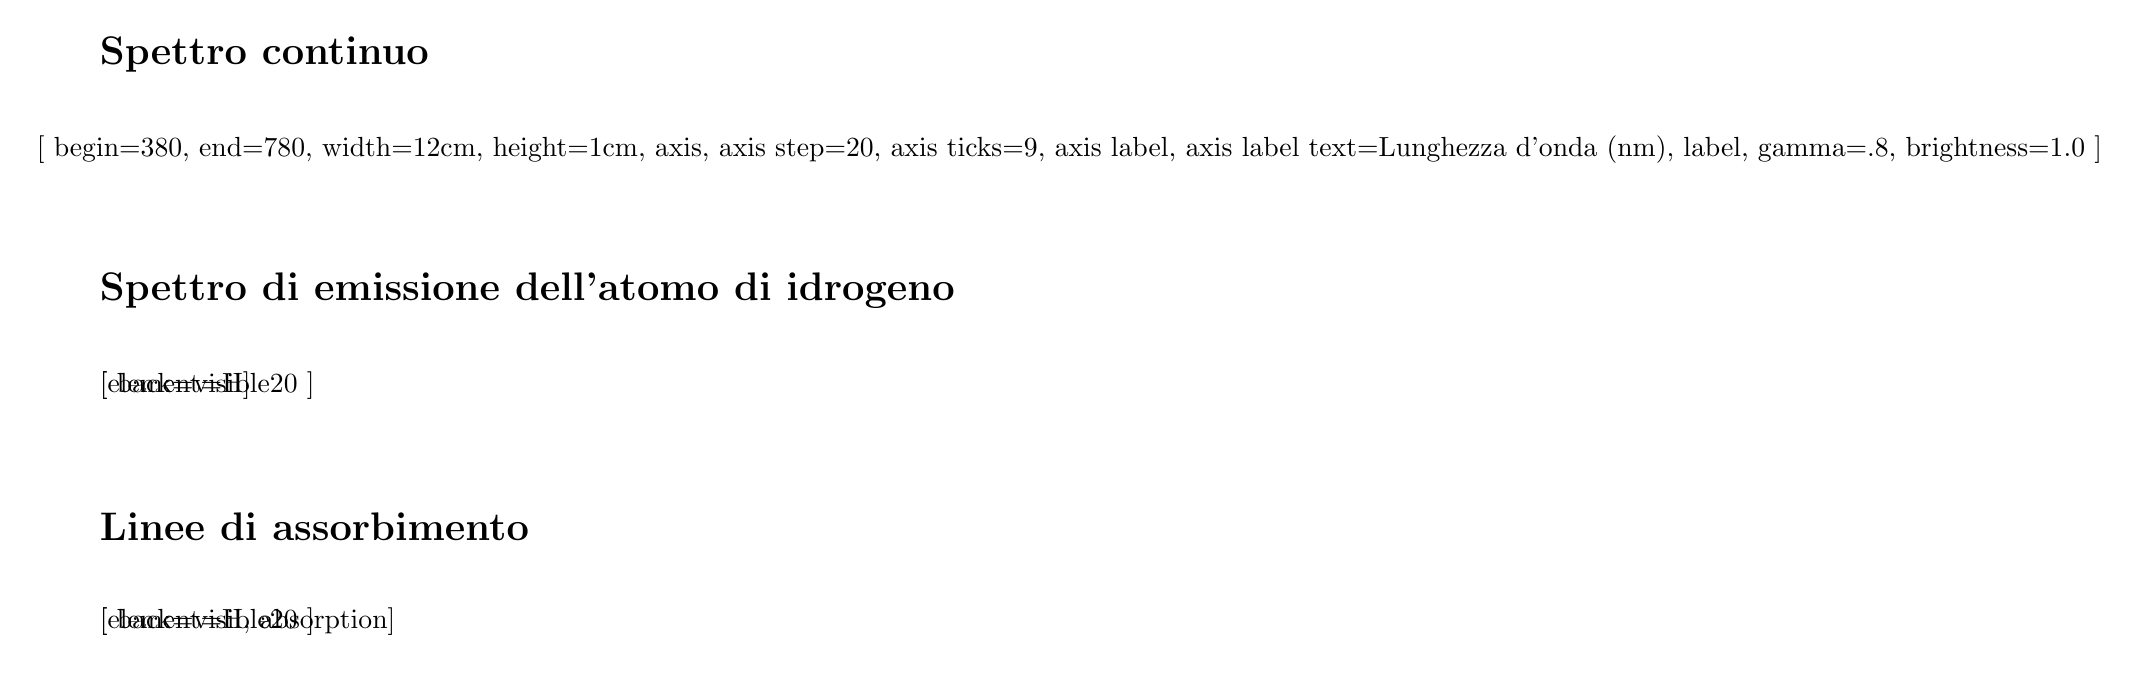
\begin{tikzpicture}

    %--------------------------
    % Parametri condivisi
    %--------------------------
    \def\W{12cm}     % larghezza barre
    \def\H{1cm}      % altezza barre
    \def\V{3cm}    % passo verticale tra pannelli (titolo + barra)
    \def\lambdaMin{380}
    \def\lambdaMax{780}

    % Stile base per pannelli con asse e label
    \pgfspectraStyle[
      axis,                   % asse delle λ
      begin=\lambdaMin,
      end=\lambdaMax,
      axis step=20,
      axis ticks=9,
      axis label,
      axis label text={Lunghezza d'onda (nm)},
      width=\W,
      height=\H,
      line width=1pt,
      gamma=.8
    ]

    % ==========================
    % PANNELLO 1: Spettro continuo
    % ==========================
    \begin{scope}[shift={(0,0)}]
      \coordinate (left) at (0,0);
      \node[anchor=west] at ([yshift=1.2cm]left) {\Large\bfseries Spettro continuo};
      % barra continua
      \node[anchor=west] at ([xshift=-0.8cm]left){%
        \pgfspectra[
          begin=\lambdaMin, end=\lambdaMax,
          width=\W, height=\H,
          axis, axis step=20, axis ticks=9,
          axis label, axis label text={Lunghezza d'onda (nm)},
          label,
          gamma=.8, brightness=1.0
        ]%
      };
    \end{scope}

    % ==========================
    % PANNELLO 2: Emissione H
    % ==========================
    \begin{scope}[shift={(0,-\V)}]
      \coordinate (left) at (0,0);
      \node[anchor=west] at ([yshift=1.2cm]left) {\Large\bfseries Spettro di emissione dell'atomo di idrogeno};

      % sfondo visibile + linee di emissione
      \node[anchor=west] at ([xshift=0cm]left) {%
        \pgfspectra[
          back=visible20
        ]%
      };
      \node[anchor=west] at ([xshift=0cm]left) {%
        \pgfspectra[element=H]%
      };
    \end{scope}

    % ==========================
    % PANNELLO 3: Assorbimento H
    % ==========================
    \begin{scope}[shift={(0,-2*\V)}]
      \coordinate (left) at (0,0);
      \node[anchor=west] at ([yshift=1.2cm]left) {\Large\bfseries Linee di assorbimento};

      % sfondo visibile + linee di assorbimento
      \node[anchor=west] at ([xshift=0cm]left) {%
        \pgfspectra[
          back=visible20
        ]%
      };
      \node[anchor=west] at ([xshift=0cm]left) {%
        \pgfspectra[element=H, absorption]%
      };
    \end{scope}

  \end{tikzpicture}
